% Booklet NLI: technical report, Hack Apertus 2026, Track 2A (OST).
% Build: make -C track_2a report   (Tectonic) -> track_2a/kaiser-data_Report.pdf
% Figures: uv run --with matplotlib python paper/figures.py (from the committed run files).
% The archival long version with every experiment is technical_report.md.
\documentclass[10pt,a4paper]{article}
\usepackage[margin=2cm]{geometry}
\usepackage[T1]{fontenc}
\usepackage[utf8]{inputenc}
\usepackage{lmodern}
\usepackage{microtype}
\usepackage{booktabs}
\usepackage{graphicx}
\usepackage{xcolor}
\usepackage{tcolorbox}
\usepackage{enumitem}
\usepackage[numbers,sort&compress]{natbib}
\usepackage[hidelinks]{hyperref}
\setlist{nosep,leftmargin=*}
\setlength{\parskip}{3pt}
\setlength{\parindent}{0pt}

% Author's own text. Remove this macro's box once the paragraph is final.
\newtcolorbox{human}[1][]{colback=yellow!12,colframe=orange!70!black,boxrule=0.4pt,
  left=4pt,right=4pt,top=2pt,bottom=2pt,fontupper=\small,title={\small Author's voice: #1},
  coltitle=black,colbacktitle=yellow!35,fonttitle=\bfseries}

\title{\vspace{-1.2cm}\textbf{Checking campaign claims against the official voting booklet}\\[2pt]
  \large Multilingual document-grounded NLI with Apertus\,v1.5 --- Hack Apertus 2026, Track 2A (OST)}
\author{Martin Kaiser (team \texttt{kaiser-data}) \quad
  \href{https://github.com/kaiser-data/hack-apertus-booklet-nli}{github.com/kaiser-data/hack-apertus-booklet-nli}\\
  \small Image \texttt{ghcr.io/kaiser-data/hack-apertus-booklet-nli:latest} \quad
  Demo \href{https://booklet-nli.pages.dev/demo/}{booklet-nli.pages.dev/demo}}
\date{\vspace{-0.8cm}}

\begin{document}
\maketitle

\begin{abstract}
\noindent Given an official Swiss federal voting booklet (German, French or Italian PDF) and a claim
in any of the three languages, our system decides whether the booklet \emph{supports},
\emph{contradicts} or \emph{does not settle} the claim, and quotes the sentences it relied on, with
pages. Apertus is the only model that decides; a small CPU embedder picks the 16 passages it reads.
On 976 held-out test claims Apertus-v1.5-8B reaches \textbf{macro-F1 0.891} (95\% CI 0.871--0.909)
with $\sim$3{,}400 prompt tokens per claim; reading the whole booklet instead scores 0.735 at
31{,}400 tokens on the same 60 claims. Under the organisers' scorer on 150 dev claims per task,
Apertus-v1.5-70B with the same pipeline and the same tokens reaches \textbf{0.905--0.925} (booklet)
and \textbf{0.979--0.986} (given passage) over two runs, against 0.857 / 0.930 for the 8B.
Quoting single sentences instead of whole pages raises the evidence score from 0.535 to 0.758.
\end{abstract}

\section{Why this matters}
\begin{human}[Q1, Q2 --- why this challenge, who uses it, in which moment]
\emph{Draft, replace with your own words:} Before every federal vote, each Swiss household receives
the Federal Council's explanations. During the campaign, voters meet claims on posters, in debates
and in their feeds, often in another language than their booklet. This system lets anyone check a
claim against what the official booklet actually says, and open the page to verify it.
\end{human}

\textbf{What we found.}
(1) \emph{Less context is more accurate}: 16 retrieved passages beat the whole booklet at a ninth of
the tokens (Fig.~\ref{fig:context}). (2) \emph{Scored evidence rewards short quotes}: the same
verdicts score 0.535, 0.616 or 0.758 depending only on how they are quoted (Fig.~\ref{fig:evid}a).
(3) \emph{Under this scoring, the larger LLM is free and the larger embedder is not}: the 70B adds
5--7 F1 points at equal tokens, because LLM latency is not charged, while embedders that retrieve
better cost 25--60$\times$ the CPU time the clock does count (Fig.~\ref{fig:evid}b).

\section{Task, data and scoring}
\textbf{Task.} Document + claim $\rightarrow$ entailment / neutral / contradiction, judged against the
booklet only, not real-world truth. All nine claim/booklet language pairs occur. The official
evaluation runs our Docker image on a private set with two tasks: \emph{A}, booklet PDF + vote name
+ claim; \emph{B}, a given reference passage + claim~\cite{starter,ostslides}.

\textbf{Data.} OST's benchmark~\cite{ostdataset} (1{,}488 pairs, balanced over labels and language
pairs). It has no split, so we split \emph{by vote date}: the three language versions of a booklet
are always on the same side. Dev: 6 dates, 512 pairs (all design choices); test: 14 dates, 976
pairs, run once. Booklets come from the Federal Chancellery~\cite{booklets}.

\textbf{Scoring}~\cite{ostslides}. A submission is valid only if macro-F1 $\geq$ 0.60 (A) and
$\geq$ 0.75 (B). Task A $=0.5\,$F1 $+\,0.2\,$evidence Hit@5 $+\,0.15\,$time $+\,0.15\,$tokens;
task B $=0.7\,$F1 $+\,0.15\,$time $+\,0.15\,$tokens; final $=0.6A+0.4B$. Tokens are counted by the
organisers' proxy; \emph{time} is wall-clock time minus the time with an LLM request in flight, so
parsing and embedding count and Apertus latency does not. Both are relative to the best team.
Evidence counts if a quote fuzzily lies inside the gold passage or contains it.

\section{System}
\textbf{Passages.} PyMuPDF extracts each page; words broken across lines are rejoined; text blocks
are merged into passages of $\leq$900 characters that never cross a page, each keeping its page
and PDF outline path (vote $\rightarrow$ part $\rightarrow$ subsection).
\textbf{Retrieval.} \texttt{paraphrase-multilingual-MiniLM-L12-v2}~\cite{reimers2020} (ONNX, CPU)
embeds claim and passages in one cross-lingual space, so a French claim finds German passages
without translation; the 16 nearest passages go to Apertus in document order.
\textbf{Verdict.} One Apertus call per case, temperature 0, JSON schema
\{\texttt{reason}, \texttt{evidence}, \texttt{label}\}; the prompt defines the three labels, names
the vote, and treats a statement attributed to the wrong actor as a contradiction.
\textbf{Evidence.} Up to five verbatim sentences with their page: the three closest to the claim
from the passages Apertus cited, then two from the rest of its context.
\textbf{Engineering for the contract.} Booklets are parsed and embedded lazily inside six worker
threads (one PDF at a time), so this work overlaps other cases' Apertus calls; answers are written
as they complete; a failing case is retried, then answered neutral, and the run always exits 0. The
image lists the endpoint's models and prefers Apertus-v1.5-70B~\cite{apertus70b}, falling back to
the 8B~\cite{apertus8b} if the 70B is not served. CI builds the amd64 image and runs it with the
network off before every publish.

\section{Results}
\begin{table}[h]
\centering\small
\begin{tabular}{@{}llccccc@{}}
\toprule
Split & Model & Task A F1 & Task B F1 & Evid.\ (A) & In tokens A / B & Out A \\
\midrule
Test, 976 (own scorer) & 8B & 0.891 {\scriptsize(0.871--0.909)} & -- & 0.716$^\dagger$ & 3{,}424 / -- & 86 \\
Dev, 150/task (official) & 8B & 0.857 & 0.930 & 0.768 & 3{,}349 / 2{,}286 & 86 \\
Dev, 150/task (official) & \textbf{70B}, run 1 & \textbf{0.925} & \textbf{0.979} & \textbf{0.808} & 3{,}349 / 2{,}286 & 92 \\
Dev, 150/task (official) & \textbf{70B}, run 2 & \textbf{0.905} & \textbf{0.986} & \textbf{0.808} & 3{,}349 / 2{,}286 & 92 \\
\bottomrule
\end{tabular}
\caption{\textbf{The 70B gains 5--7 points on the booklet task at identical input tokens.}
``Official'': the organisers' \texttt{evaluate.py}~\cite{starter} on cases in their format, run in our
Docker image on Modal. $^\dagger$Test evidence uses our own n-gram overlap measure, not the official
matcher. Run 2 let the image choose the model itself. An identical 8B rerun differs by up to 0.027
(\S\ref{sec:limits}). Files: \texttt{runs/test-rag-k16-n976/}, \texttt{runs/contract-dev-n150/}.}
\label{tab:main}
\end{table}

\begin{figure}[h]
\centering
\begin{minipage}[t]{0.47\linewidth}\vspace{0pt}
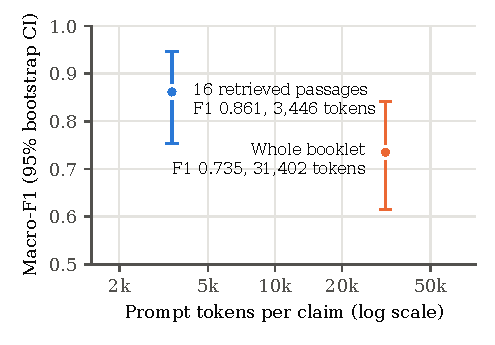
\includegraphics[width=\linewidth]{fig-context.pdf}
\end{minipage}\hfill
\begin{minipage}[t]{0.5\linewidth}\vspace{4pt}
\caption{\textbf{Reading less of the booklet is both cheaper and more accurate.} The same 60
held-out test claims, Apertus-v1.5-8B. The whole booklet costs 9$\times$ the tokens and six of its
60 answers never finish: the model lists passage numbers until the output cap. Retrieval leads by
+0.127 counting those as neutral, +0.053 (CI $-$0.056 to +0.168) excluding them. Bars: 95\%
bootstrap intervals over claims. Source: \texttt{paper/figures.py} on
\texttt{runs/test-full-n60}, \texttt{runs/test-rag-k16-n976}.}
\label{fig:context}
\end{minipage}
\end{figure}

\begin{figure}[h]
\centering
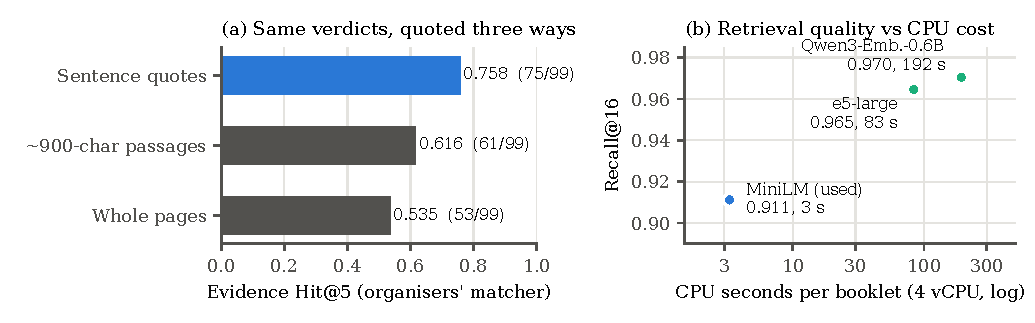
\includegraphics[width=\linewidth]{fig-evidence-embedders.pdf}
\caption{\textbf{(a) The scorer rewards short quotes; (b) better retrieval costs counted CPU time.}
(a) Identical 8B verdicts on 99 non-neutral dev claims, quoted as whole pages, our passages, or
sentences, scored by the official matcher: a gold passage often includes a heading that a page does
not reproduce contiguously, so the page does not ``contain'' it. (b) Recall of the annotated passage
in the top 16 (338 dev claims) against CPU seconds to embed one booklet on 4 vCPU:
multilingual-e5-large~\cite{wang2024e5} and Qwen3-Embedding-0.6B~\cite{zhang2025qwen3emb} retrieve
better but cost 83 and 192\,s per booklet, against 3\,s, time the official clock counts. Fusing BM25
by reciprocal rank~\cite{robertson2009bm25,cormack2009rrf} did not help at $k=16$ (0.905 vs 0.911).
Source: \texttt{modal/embed\_bench.py} $\rightarrow$ \texttt{runs/embed-bench-dev.json};
\texttt{runs/contract-dev-n150/evidence-variants/}.}
\label{fig:evid}
\end{figure}

\textbf{Languages.} On test, cross-lingual pairs score 0.899 (n = 641) and same-language pairs
0.875 (n = 335); booklet DE 0.866, FR 0.898, IT 0.908. We see no sign that translation is needed.
\textbf{Errors.} Contradiction predicted as neutral is the main confusion (31 of 106 test errors).
Retrieval misses explain only 26 of the 106: in 44 of the 70 claims whose annotated passage was
not retrieved, the verdict was still correct from other passages. Given the annotated passage (task B), the 8B scores 0.930
against 0.857 with retrieval: most remaining errors happen with the right text in hand.
\textbf{Efficiency.} Task A uses 3{,}349 input tokens per case (task B 2{,}286, mostly the reference
itself); the median Apertus response is 4.5\,s (8B, test). With lazy preparation, the
time with no request in flight was below 1\,s for 300 mixed cases; [A-only measurement pending].

\section{What we learned}
\begin{human}[Q4--Q8 --- the decisions, told by you]
\emph{Draft, replace:} Our first instinct --- and that of another AI we asked --- was to cite whole
pages, since a page ``contains'' the passage. Measuring with the organisers' matcher showed the
opposite. The same happened with the embedder: the state-of-the-art models are better, and we kept
the small one because the rules charge CPU time. And the night before the deadline we switched to
the 70B, because under these rules a larger LLM costs nothing but its GPU bill. The common thread:
read the scorer before trusting intuition.
\end{human}

\section{Limitations and ethics}\label{sec:limits}
\textbf{Noise.} An identical 8B rerun on dev moved macro-F1 by 0.027 (batched GPU inference is not
bit-exact at temperature 0, and near-tied passages reorder); dev decisions rest on 6 vote dates, and
differences below $\sim$0.03 are ties. The 70B result rests on two dev runs, not on the test split.
\textbf{Evidence.} Hit@5 is a proxy; the last two quotes come from retrieved context the model did
not cite (the demo shows only cited passages). \textbf{Scope.} One booklet may cover several votes;
retrieval can pick the wrong one. \textbf{Ethics.} A verdict says what the booklet states, not
whether a claim is true or how to vote; it is a model prediction to check against the cited page,
not political advice. No personal data is processed.

\section{Use of AI}
\begin{human}[Q12 --- confirm or correct this list]
\small
\begin{tabular}{@{}p{0.25\linewidth}p{0.67\linewidth}@{}}
Apertus-v1.5-8B / 70B & the only model in the system that decides labels and cites evidence \\
MiniLM (multilingual) & passage retrieval only; e5-large and Qwen3-Embedding were benchmarked, not used \\
Claude Code (Anthropic) & wrote most of the code and these documents under the author's direction; ran experiments on Modal \\
Codex CLI (OpenAI) & five read-only reviews (12 Oct twice, 13 Oct, 15 Oct twice); every finding checked against the code before acting \\
Grok (xAI) & two read-only reviews of data and results (12 Oct) \\
\end{tabular}
\end{human}
All numbers in this report are recomputed from committed run files; no AI-generated number entered
the report without that check.

\section{Reproducibility}
Code, run files and every prediction: the repository above (Apache-2.0); dataset pinned to revision
\texttt{fc2b276}; temperature 0, seed 0. Apertus served with vLLM~\cite{kwon2023vllm} on Modal (8B: one
L40S; 70B: two H200, tensor parallel). Official contract:
\begin{center}\small\texttt{docker run -e BASE\_URL -e API\_KEY -v <cases>:/data:ro -v <out>:/output <image>}\\
\texttt{--input /data/cases.jsonl --output /output/predictions.jsonl}\end{center}
Every experiment, including rejected ones
(prompt changes, parser v4, vote routing, a k=8$\rightarrow$16 cascade), is documented in
\texttt{technical\_report.md}, the archival long version.

\begin{human}[Q10, Q11 --- next step and the sentence to remember]
\emph{Draft:} Next, an actor-aware verifier that states who claims what before the label, tested on a
challenge set where only the speaker, number or negation changes.
\end{human}

\small
\bibliographystyle{unsrtnat}
\bibliography{refs}
\end{document}
